\documentclass[letter, USenglish, 11pt, subfigure]{article}
\usepackage[margin=1in]{geometry}
\newcommand*{\ATLASLATEXPATH}{./}
\usepackage{\ATLASLATEXPATH atlaspackage}
\usepackage{\ATLASLATEXPATH atlasbiblatex}
\usepackage{\ATLASLATEXPATH atlasphysics}
\usepackage{\ATLASLATEXPATH ANA-SUSY-2018-12-PAPER-defs}
\usepackage{enumerate}
\usepackage{caption, float, threeparttable}
\newcommand{\tth}{\ensuremath{\ttbar H}}
\newcommand{\ttH}{\ensuremath{\ttbar H}}
\newcommand{\tthyy}{\ensuremath{\ttbar H(\to\gamma\gamma)}}
\newcommand{\myy}{\ensuremath{m_{\gamma\gamma}}}
\newcommand{\hyy}{\ensuremath{H(\to\gamma\gamma)}}

\usepackage{lineno}

\linenumbers
\usepackage{wrapfig}
\usepackage{placeins}
\usepackage{pdfpages}
\usepackage[none]{hyphenat}

\usepackage{xifthen}
\usepackage{multirow,bigdelim,makecell}
\usepackage{cellspace}
\usepackage{selectp}
\usepackage{color, colortbl}

% \outputonly{1}
\usepackage[nottoc,numbib]{tocbibind}

\addbibresource{proposal_WHopkins.bib}
\addbibresource{ATLAS-SUSY.bib}
\addbibresource{ATLAS.bib}
\addbibresource{ANA-HDBS-2021-10-PAPER.bib}
\addbibresource{CMS.bib}

\pagestyle{headings}

\title{Early Career Research Proposal: \\Enabling Calibrations of Machine Learning Approaches (ECMLA)}
\author{Applicant/Institution: Walter Hopkins, Argonne National Laboratory\\ Postal Address: \\Argonne National Laboratory, 9700 S. Cass Avenue, Building 360, Lemont, IL 60439
  \\PI name: Walter Hopkins\\Position title for PI: Physicist\\PI telephone number, email: (630) 252 7551, whopkins@anl.gov\\Administrative Point of Contact name, telephone number, email:\\Diane Hart, (630) 252 7677, dhart@anl.gov\\FOA Number: DE-FOA-0003176\\DOE/SC Program Office: HEP\\ Topic Area: Experimental Research at the \\Energy Frontier in High Energy Physics\\DOE/SC Program Office Technical Contact: Abid Patwa\\Year Doctorate Awarded: 2013\\Number of Times Previously Applied: 2\\Eligibility Extension Requested: No
}
\date{}

\begin{document}
\pagenumbering{gobble}
% \includepdf{cover_page_signed.pdf}

% \maketitle
\clearpage
\tableofcontents
\thispagestyle{empty}

\clearpage
\pagenumbering{arabic} 
\section{Introduction}

Machine learning (ML) has increasingly become a critical tool in High-Energy Physics (HEP), offering significant advancements in various tasks such as simulating calorimeter showers, identifying particles, and distinguishing between signal and background processes. ML techniques allow physicists to delve into complex correlations among a wide range of observables, from the trajectories and energies of particles to their interactions within detectors. 

However, the application of ML in HEP is accompanied by certain challenges that need careful consideration. One such challenge is the alignment of input variable distributions between Monte Carlo (MC) simulations and experimental data. Differences between MC simulations and recorded data can introduce additional uncertainties into ML predictions, affecting the overall systematic uncertainties in physics measurements. Additionally, ML algorithms may be sensitive to experimental systematic uncertainties which are typically assessed by varying underlying experimental parameters (e.g., the energy resolution of a subdetector). Furthermore, ML models can sometimes create unintended correlations between their outputs (such as estimated energy or particle identification) and other variables critical for calibrations or background estimations.

Recently proposed ML approaches such as adversarial~\cite{louppe2017learning} and distance correlation (DisCo)~\cite{PhysRevLett.125.122001} techniques have shown promise in various applications such as reducing uncertainties in a long-lived particle search~\cite{calRatio} and decorrelating jet substructure variables from jet mass~\cite{ATL-PHYS-PUB-2018-014}.
These approaches are part of a group of methods that aim to improve the ``domain adaptation'' of ML algorithms, i.e., the ability of an ML model trained with one set of data to be robust enough to be applied to data that is expected to be different from the training data. Domain adaptation techniques have the potential to be more broadly applied when developing ML models to estimate physics object properties (e.g., photon energy, jet transerve momentum, etc), to identify (ID) physics objects (e.g., photons, jets containing $b$-hadrons, etc), to reduce the sensitivity data-MC discrepancies, detector and accelerator conditions (e.g., the number of simultaneous proton-proton interactions, pile-up), and to changes in the underlying parameters of simulations. All these applications of domain adaptation approaches could reduce the total uncertainties of physics results within HEP. 

This proposal presents {\bf the development of a framework to deploy various domain adaptation techniques to minimize uncertainties when using machine-learning-based physics object ID and property estimation by ensuring that ML models are more resilient against experimental systematic uncertainties, data-MC differences, and changes in detector conditions. Furthermore, the PI's team intends to refine domain adaptation methods that generate durable features, less affected by specific assumptions (such as detector resolution and pile-up), that have not been previously applied in HEP, for implementation in HEP contexts. } The framework has broad applications but will first be used to maximize object ID efficiencies and property estimation precision. The proposed techniques could also improve object ID and property evaluations (potentially improving both the efficiency and resolution) at the trigger level, especially given the recent work on fast inference on field-programmable gate arrays (FPGAs).

Improving both ID efficiencies (which is equivalent to recording more data) and reducing systematic uncertainties will be essential to enabling future discoveries in collider physics. Results from the Large Hadron Collider (LHC) experiments have verified the predictions of the highly successful Standard Model (SM), culminating with the discovery of the Higgs boson~\cite{HIGG-2012-27,CMS-HIG-12-028}. However, the SM  lacks an explanation for several observed phenomena (e.g., dark matter, the matter-antimatter asymmetry, etc) motivating the search for Beyond the Standard Model (BSM) physics. Future LHC upgrades will no longer include substantial increases in energy and move HEP into the precision era, with a tenfold increase (High Luminosity-LHC, HL-LHC) of the Run~2 dataset. 

Precision measurements of SM processes, especially interaction involving Higgs bosons, can probe for BSM effects resulting from particles which may have large masses that prevent them from being directly produced at the LHC. An essential aspect to improving the precision of measurements, which will maximize sensitivity to BSM physics, is the calibration of physics object ID and properties. This calibration involves evaluating ID efficiencies and properties in MC simulations and correcting these quantities to the true property before reconstruction or to what is observed in data. 

The Higgs boson self coupling and the coupling to the top quark are especially sensitive to BSM effects~\cite{Agrawal_2020}. The associative production of a top quark pair with a Higgs boson (\tth) is sensitive to both of these couplings~\cite{Maltoni_2017} and thus the \tth\ total and particularly differential cross-section measurements, e.g., as function of Higgs \pt, can serve as probes for BSM physics. The latest ATLAS \hyy, which includes \tthyy, differential cross-section results~\cite{ATLAS_STXS} remain limited by the statistical uncertainty in each kinematic observable bin. However, the photon ID and energy resolution uncertainties are the dominant detector-based systematic uncertainties and are currently on par with the other dominant source of systematic uncertainty, theory uncertainties. Reducing these detector systematic uncertainties will become significantly more important for all \hyy\ measurements, as ATLAS drastically increases the size of its dataset near the end of HL-LHC data taking. Thus, the unprecedented data volume of the HL-LHC offers an opportunity to improve the precision cross-section measurements as a function of kinematic variables in channels with high \tth\ purity, i.e., where the Higgs decays to two photons (\tthyy).

The proposed framework and techniques will first be developed and applied to photon ID and energy resolution because these are key ingredients to maximizing the sensitivity of Higgs precision measurements. Studies have been performed within ATLAS that showed a potential $\sim$10-20\% improvement in both ID efficiency (which is equivalent to collecting 10-20\% more data) and energy resolution when including all available information for ID and energy estimation. However, as soon as the calibration of the ID efficiency and energy resolution was taken into account, the gain in efficiency and enhancement in resolution were lost. For the ID, ML approaches were found to be correlated with quantities that needed to be independent of the ID for the calibration while for the energy resolution it was found that ML methods were sensitive MC mismodelling of shower shapes. Thus, {\bf the proposed domain adaptation techniques could improve all ATLAS measurements involving $H\to\gamma\gamma$ which are essential to the HL-LHC BSM search program.}

The PI's experience in ML, e.g., as one of the ATLAS ML Forum conveners and a co-developer of unsupervised learning techniques for use in ATLAS, as well as his experience with the LAr calorimeter and calorimeter simulations will aid the success of this proposal. The PI will also draw from his work within the ATLAS SUSY group, as a leader of flagship searches~\cite{stop0L_1,stopRun1,stop0L_2,stop0L_3} involving $\ttbar$ final states. 


\subsection{Domain Adaptation for HEP Machine Learning Models}

Machine learning has already been used for the identification of various physics objects (i.e., electrons, jets containing b-hadrons, etc) and to calibrate properties of objects (e.g., for pions~\cite{ATL-PHYS-PUB-2020-018}). Many of these ML models, however, use simulations for training and do not automatically take data-MC differences into account during training. Additionally, algorithms may be required to be independent from variables that are either used in part of the calibration procedure, e.g., to determine the rate of fake objects~\cite{atlas_photon_id}, or that might vary during the operations of the collider or detector, e.g., pile-up which will be particularly challenging environment at the HL-LHC. Improving the robustness of ML models used to identify and calibrate objects so that these effects are mitigated will have far reaching impacts on physics results.

There have been recent advancements in using domain adaptation techniques to decorrelate ML models from certain quantities (e.g., the output of an ML model that summarizes jet substructure that is not correlated to jet mass) using methods such as adversarial discriminants and distance correlation. Adversarial approaches involve two ML models, one that generates high-dimensional distributions and another model that is trained to discriminate between the ML-generated data and the real data. More recently, adversarial approaches have been used to discriminate between recorded and simulated data from the output of another discriminator~\cite{calRatio}. This strategy, i.e., to impose penalties on an ML model for producing inconsistent results across various datasets, can be applied to minimize differences between data and MC or between MC datasets with different parameter values (e.g., the energy resolution of jets). This is achieved by including two optimization quantities (i.e., cost or loss functions), one for each ML model. Using two opposing ML models to improve domain adaptations allows for complex multi-dimensional correlation to be taken into account. However, this dual-faceted optimization process, introduces a significant computational demand and presents challenges in establishing definitive criteria for the cessation of training.
% make GAN diagram
% Encoder in Autoencoder diagram

An alternative method that requires less computing resources, but may not be able to take advantage of as much information as adversarial approaches, is using distance correlation which summarizes the dependence of sets of variables. Unlike the more frequently used measure of the Pearson correlation coefficient, which can only detect linear correlations, distance correlation is sensitive to non-linear correlations, which are commonly present in HEP datasets. The distance correlation is zero only and only if there are no correlations between the input variables. This feature allows it to easily be added to typical loss functions which are minimized to optimize ML models. Thus, distance correlation is simpler to implement than adversarial techniques with less hyperparameter (since only a loss term is added rather than an entire NN) and more stable training characteristics. 

Another, less explored within HEP, domain adaptation technique is feature representation transfer. The idea is to learn a feature representation that is domain-invariant. Techniques such as autoencoders networks (which take inputs and encode them into a lower-dimensional space) can be used to learn such representations where the model minimizes the difference between the source and target domain features, making the model's predictions less dependent on the domain-specific features. The advantage of feature representation transfer over distance correlation and the adversarial techniques described in the previous paragraphs is that the resulting domain-adapttive features can be used for a variety of tasks. These features would be akin to physicist developed variables that are ratios of quantities that behave similar after a change in assumption (e.g., both the numerator and denominator increase at a similar scale if an energy scale is changed).

Domain adaptation allows ML models to maximize the use of all information while avoiding regions of kinematic phase space that are poorly modelled in simulation or to ensure an ML model is independent of a quantity, such as pile-up or isolation. Depending on the particular application, adversarial, autoencoder based feature representation learning, or distance correlation approaches can be the optimal solution and all should be studied when developing a particular ML model. The rise of ML-focused High-Performance Computers (HPCs), such as Aurora at the ALCF, are an opportunity to deploy these domain adaptation approaches, which can be compute intensive, across applications in HEP.

Recently, ML frameworks that are multi-modal, i.e., they can handle various types of input data (e.g., particle trajectories, jets, etc) and that are multi-task, that is they can build complex ML models for various tasks (e.g., identifying jets which contain hadrons that are initiated charm or bottom quarks, jet energy calibration, etc). SALT~\cite{salt}, is such a framework developed within ATLAS. These frameworks are powerful tools but lack infrastructure to automatically produce models that are robust against data-MC mismodelling, experimental systematic uncertainties, or pile-up. Incorporating domain-adaptation techniques within SALT will reduce systematic uncertainties which will propagate through to many ATLAS physics results.

\subsection{Initial Applications of Domain Adaptation: Photon ID and Energy Calibration}

Machine-learning-based photon ID techniques (a boosted-decision-tree, BDT) have been studied within ATLAS demonstrating a potential gain in signal efficiency of 5-10\% (e.g., moving from 88\% to 95\% efficiency for unconverted photons with \pt$\sim$60 GeV) resulting in an increase of statistics of 10-20\% (thus reducing the statistical uncertainty by 10-17\% for events with two photons) while retaining the same background rejections as the current rectangular-requirement-based ID. An increase in efficiency would impact all $H\to\gamma\gamma$ measurements by improving the statistical power of these measurements with the same amount of HL-LHC data while increasing the background rejection (once the signal efficiency has saturated) will result in an even purer $H\to\gamma\gamma$ signal. Even more efficiency gains and increased background rejection have been observed when using convolutional neural networks (CNNs). However, photon ID calibration procedures and fake-photon background estimation techniques used in many ATLAS analyses necessitates that the photon ID is uncorrelated from track isolation (a measure of the energy associated with the candidate vs the energy around the candidate). This requirement of orthogonality to particular quantities has limited the use of ML for photon ID within ATLAS. Additionally, the Phase II upgrade of the ATLAS Inner Tracker (ITk) will improve the track isolation, which yields an opportunity to revisit the ATLAS photon ID and its calibration to maximize performance during the HL-LHC. 

The calibration of photon energies was studied using both advanced ML architectures, i.e., CNNs and graph neural networks (GNNs), and more information than the current BDT-based algorithm used. The resulting calibration showed a $\sim$20\% improvement in photon energy resolution but was sensitive to data-MC mismodelling in variables that summarized the shape of the energy deposits in the calorimeter. Ensuring that ML models are invariant with respect to these mismodelled quantities could result in significantly improved photon energy resolution which in turn will reduce the systematic uncertainties for analyses that include photons in their final states (which includes all channels that involve $H\to\gamma\gamma$ decays such as the Higgs mass measurement).

\clearpage
\subsection{Precision Differential Cross-Section Measurements at the HL-LHC}
The HL-LHC will deliver a very large HEP datasets yielding opportunities to perform new measurements and with unprecedented precision.
Many measurements which were statistically constrained will become systematic uncertainties which will underscores the pivotal role of systematic uncertainties in shaping the landscape of precision measurements within the HEP. There are, however, measurements with potentially significant BSM contributions that will benefit from an increase of the dataset size. Such an increase is only possible by improving the ID efficiency of physics objects that are expected to be present in various final states. 

Measurements involving the SM Higgs become increasingly sensitive to high mass BSM contributions as the precision of measurements improves. As the size of the LHC dataset grows, differential cross-section measurements, which can further expose the effects of BSM physics in high-energy regions (see Figure~\ref{fig:SMEFT_highmass} for an illustration of this effect), become more powerful tools in the search for BSM physics.
The results of differential cross-section measurements can probe BSM effects by being interpreted in the context of the Standard Model Effective Field Theory (SMEFT)~\cite{Buchmuller:1985jz,Grzadkowski:2010es,SMEFTsim3} and in the case of Higgs-related measurements, results can also be interpreted in terms of coupling strengths within the $\kappa$-framework~\cite{deFlorian:2016spz}.
\begin{wrapfigure}{l}{0.45\textwidth}
  \centering
  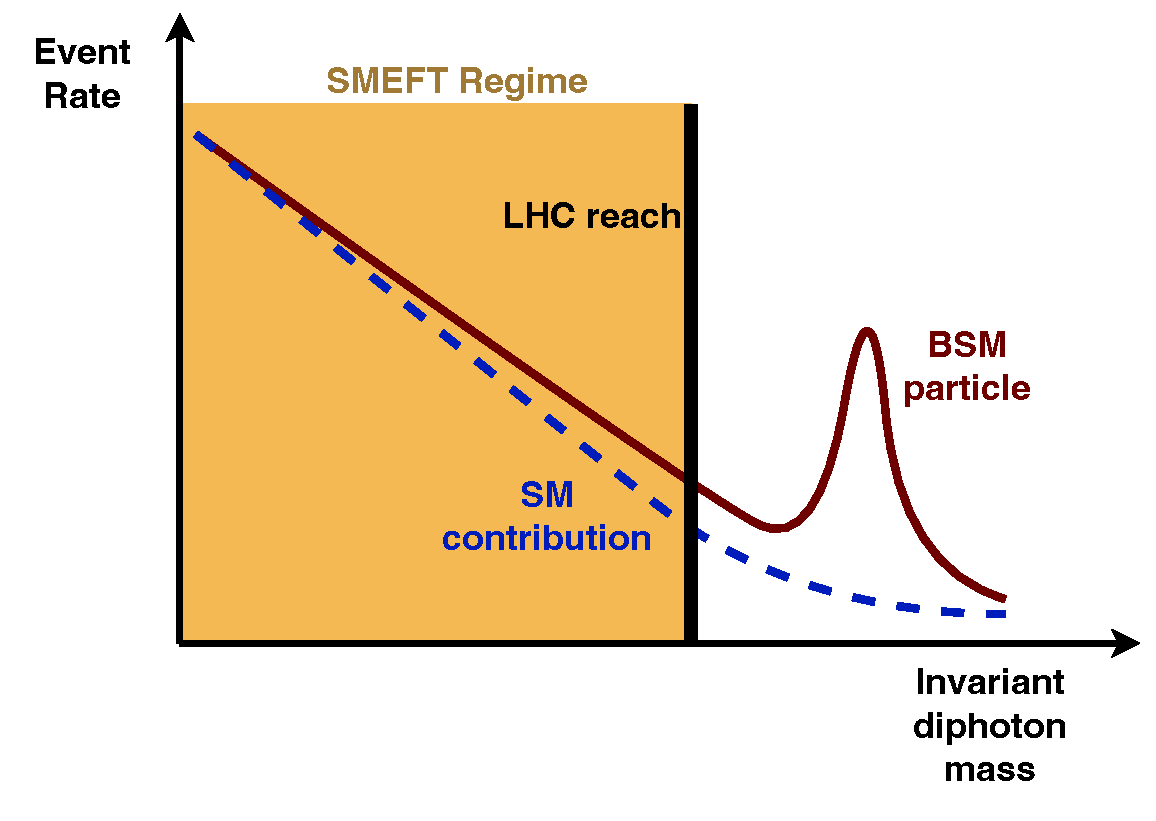
\includegraphics[width=\linewidth]{figures/SMEFT.pdf}
  \caption{\label{fig:SMEFT_highmass} Example of how effects of a heavy BSM particle can leak into high-energy regions of distributions measured at LHC experiments.}
\end{wrapfigure}
An example of a recent differential cross-section measurement involving the decay of the SM Higgs to two photons~\cite{ATLAS_STXS} used the simplified cross-section template (STXS) method, which performs measurements in bins in several kinematic dimensions (see Figure~\ref{fig:ggH_STXS}) to constrain BSM effects. Current measurements are statistically limited but have substantial systematic uncertainties (up to $\sim$40\% in one of the differential cross-section bins). For many of these measurements photon resolution and ID are some of the largest experimental uncertainty~\cite{ATLAS_STXS}. The HL-LHC will deliver a large dataset that will remove statistical limitations in most bins and thus the reduction in systematic uncertainties will have a more significant impact. However, bins in the high-energy regions, such as bins that measure properties of a Higgs being produced in association with a top pair ($\ttbar H$) will still be statistically limited with the current physics object ID efficiencies. Improving the photon ID efficiency could reduce the statistical uncertainties by up to 17\% for final states that include two photons. This improvement, however, requires work to ensure that the photon ID is uncorrelated to track isolation. The methods (i.e., distance correlation and adversarial techniques) that will be incorprated in 
the proposed framework can be applied to a new ML-based photon ID algorithm to potentially achieve the increased statistical power in topologies with two photons.

\begin{figure}[!htbp]  
  \centering
  \subfigure[ggF]{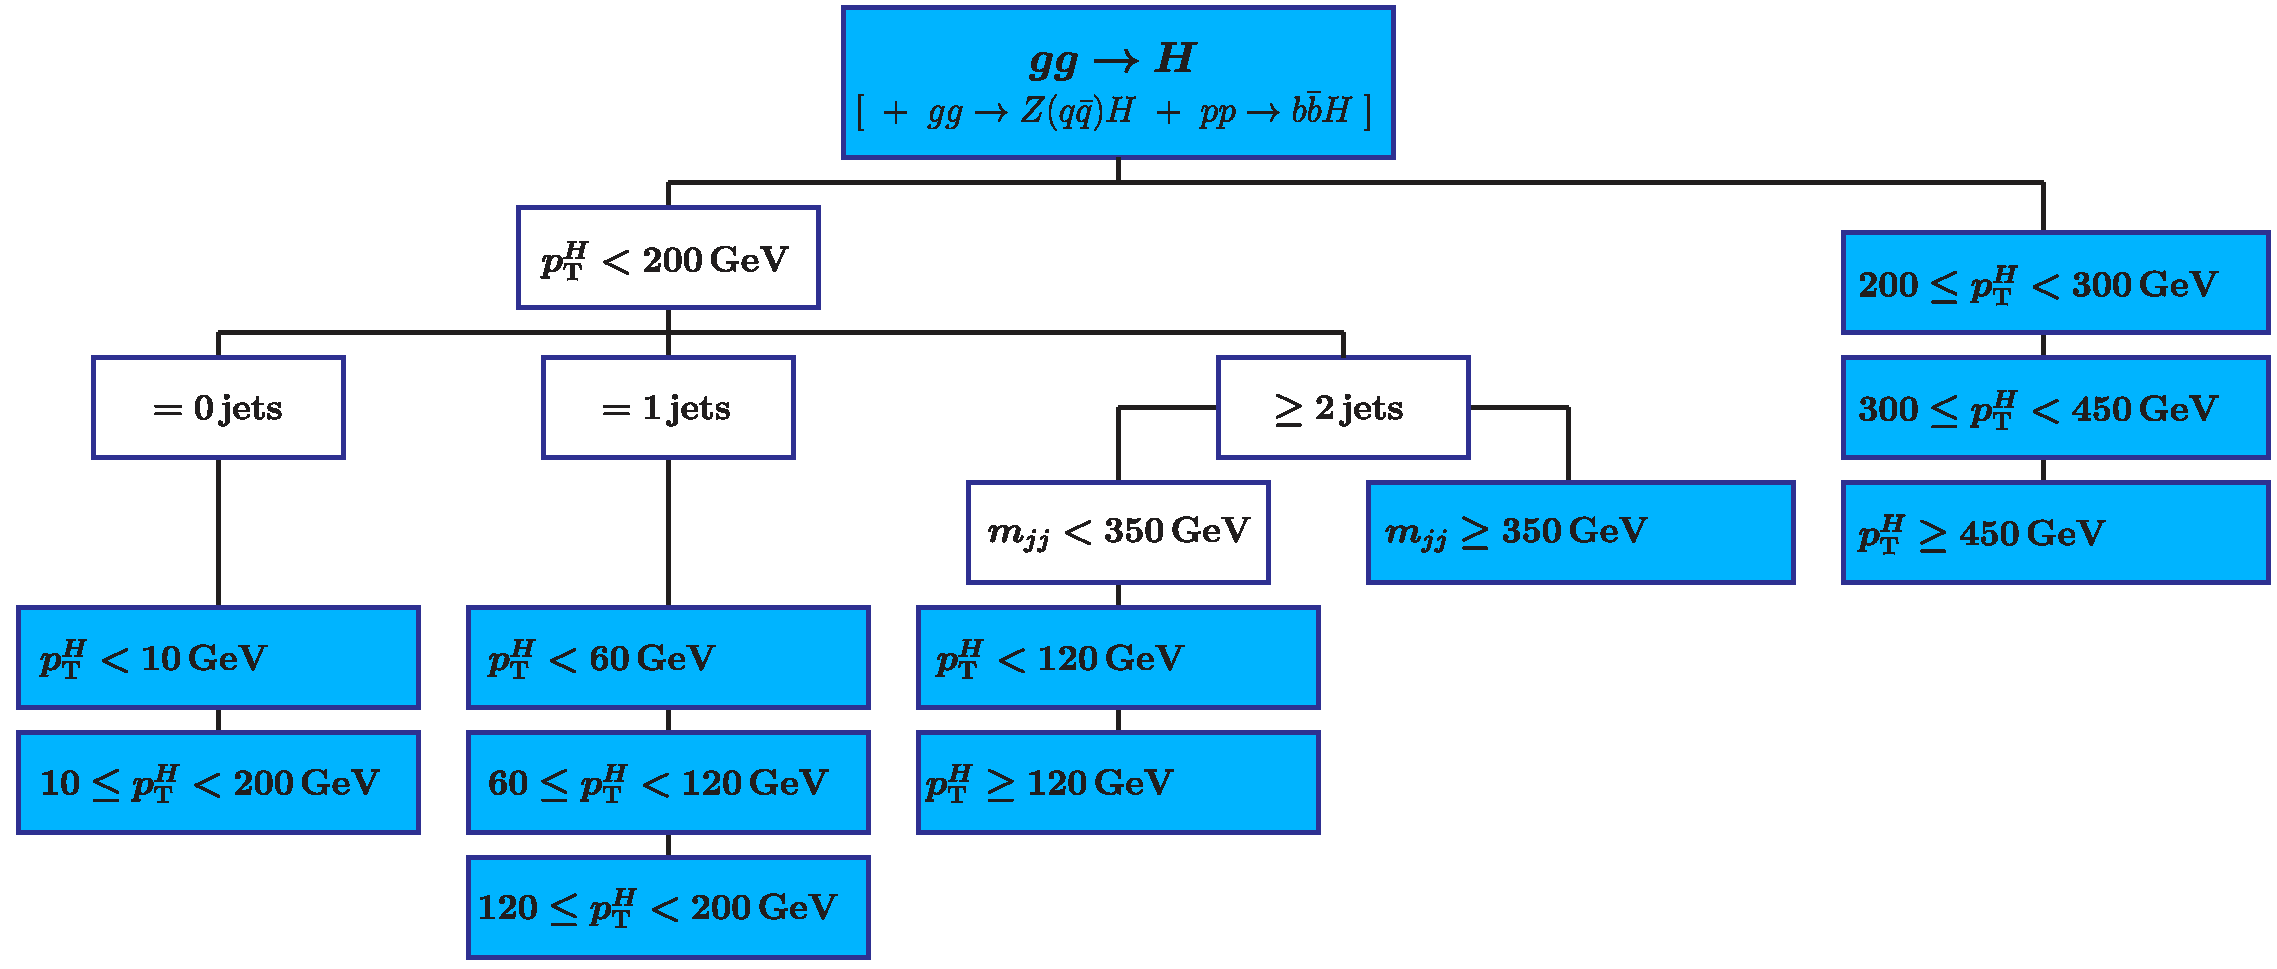
\includegraphics[width=0.8\textwidth]{figures/ggH_STXS.pdf}}
  \caption{\label{fig:ggH_STXS} Bins used in the most recent $H\to\gamma\gamma$ differential cross-section measurement.}
\end{figure}

\section{Project Objectives}
The objective of the proposed work to gain experience and fine tune three domain adaptation approaches, i.e., distance correlation, adversarial models, and feature representation transfer, for calibration tasks. An additional objective is to integrate domain adaptation techniques into ATLAS physics object ID and calibration frameworks such as ``SALT''~\cite{salt}. These approaches can help incorporate calibration considerations (e.g., differences between recorded data and simulation) into ML models which will result in a decrease in uncertainties. This will maximize the power of precision measurements by improving physics object ID and energy evaluation. This approach will first be applied to the ATLAS photon ID and energy resolution calibration which will in turn be used in the upcoming \hyy, focusing on \tthyy, differential cross-section measurements. The proposed domain adaptation techniques will also be used in the optimization of \hyy\ measurements by ensuring that final multivariate analysis (MVA) uncorrelated from the background $\gamma\gamma$ invariant mass spectrum. 

\begin{itemize}
\item Study the application domain adaptation techniques to calibrate photon ID efficiency and photon energy
  \begin{itemize}
  \item Apply established techniques (distance correlation and adversarial)
  \item Develop new technique: feature representation transfer
  \end{itemize}
\item Perform updated \tthyy\ differential cross-section measurement
  \begin{itemize}
  \item With improved photon ID and energy resolution
  \item Using new multivariate analysis which is uncorrelated from the $\gamma\gamma$ invariant mass spectrum
  \end{itemize}
\item Integrate domain adaptation techniques into existing ATLAS ML frameworks
\end{itemize}
\clearpage
\section{Proposed Research and Method}
% Gordon's talk on training with variables  https://indico.in2p3.fr/event/30589/contributions/130476/attachments/81700/120373/2023-11-30%20Using%20Adversaries%20to%20Control%20Systematics.pdf

The PI's team, consisting of two postdocs at 2.0 FTE, will customize and deploy domain adaptation techniques within an ATLAS common framework, i.e., SALT. These techniques will first be applied to improve photon energy evaluation and photon ID. The more established approaches, distance correlation and adversarial networks, will be studied in parallel with the feature representation transfer. One postdoc will gain expertise in photon energy evaluation while the other postdoc will work on photon ID using the same ML domain adaptation methods. Both postdocs will contribute to developing feature representation transfer and will work on preparing the next two iterations of the $H\to\gamma\gamma$ differential cross-section measurement.

Domain adaptation techniques will first be applied in conjunction with BDTs and will then be adapted to be used with more advanced networks such as GNNs. The adversarial approaches as well as GNNs require significant computing resources to train and tune. The PI will leverage both computing resources and expertise at Argonne to develop domain adaptive models.
The team will assess the effectiveness of domain adaptation techniques by examining residual correlations and comparing the performance of ML models with and without domain adaptation. Upon successful validation and integration of these techniques into SALT, the PI's team will with members of the Argonne ATLAS group (who will not be funded by this proposal, if awarded), who are working within the ATLAS flavor tagging group, to implement the domain adaptation approaches for flavor tagging.

In parallel to preparing domain adaptation for use in ATLAS physics object ID and property assessment, the PI's team will contribute to two differential cross-section measurements of $H\to\gamma\gamma$: an intermediate analysis using a subset of Run 3 data, and a comprehensive final result utilizing the entire dataset. The improved photon energy evaluation and ID calibrations will be used with the full Run 3 $H\to\gamma\gamma$ measurement. The PI's team will focus on ensuring that the MVA used for signal-background separation does not sculpt the diphoton mass (an essential ingredient to the background estimation) which will benefit measurements in all the bins of this diifferential cross section measurement. The PI's team will focus on the \tth\ measurement drawing from previous experience with final states that include $\ttbar$ within Supersymmetry searches and more recently, final states that include two photons within a charged Higgs search. 


\subsection{Photon-Energy Calibration}

The calibration of photon and electron energy involves several steps as detailed in~\cite{atlascollaboration2023electron}. This proposal aims to test and enhance the MC-based calibration that utilizes variables derived from energy deposits grouped in the calorimeter. The process aims to adjust for energy that is lost in material before the calorimeter, deposited in adjacent cells, or not captured by the LAr calorimeter. The current algorithm uses a BDT to regress the corrected photon energy using shower-related variables that summarize shower properties (see Figure~\ref{fig:showerVars}). The BDT is trained with a single particle MC with a flat transverse momentum (\pt) spectrum up to 150 GeV. The performance of the BDT is then evaluated by comparing the energy predicted by the BDT with the true particle energy. Internal ATLAS studies have shown that adding lateral shower shape variables to the BDT could improve the energy resolution after calibration by 10-15\%. However, these variables are poorly modelled by the simulation when compared to recorded data, preventing them from being used in the calibration. The application of domain adaptation techniques—such as integrating real data during training, reweighting training datasets to better reflect actual data distributions, employing adversarial methods, and using distance correlation strategies—could potentially reclaim some benefits of including shower shape variables, despite the discrepancies between simulation and actual data.

\begin{figure}[ht]
  \centering
  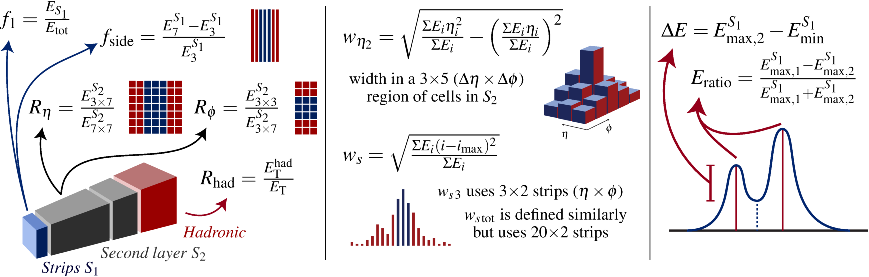
\includegraphics[width=\textwidth]{figures/photon_ID_variables.pdf}
  \caption{\label{fig:showerVars} }
\end{figure}

Two domain adaptation methods, which have already been applied within other contexts within HEP will be studied in parallel, first on the photon-energy calibration using the existing BDT energy regression, and then using a more advanced approach that utilizes GNNs and low-level calorimeter information. The PI's team will apply the adversarial and distance correlation approaches studied by the PI on a simplified toy example using the existing BDT. One postdoc will focus on the adversarial technique while the other will focus on the distance correlation approach, each at 0.5 FTE. The existing BDT has been extensively studied for various improvements and will serve as a benchmark to ensure that the domain adaptation techniques do not effect the original ML algorithm in a negative way.

The PI's team will first, together with ATLAS $e/\gamma$ experts, produce a simulation dataset that has been modified to resemble the data. This ``fudged'' MC will allow for more control of properties such as photon purity, energy scale, and sample size for initial studies; the team will also study the use of recorded data during training after the domain adaptation techniques reach a mature state. The team will use the previously developed toy model as a basis to develop domain adaptation techniques for the energy regression BDT. As a former convener of the ATLAS Full Simulation group, which aims to improve both the physics and computational performance of the ATLAS detector simulation based on GEANT4~\cite{Agostinelli:2002hh}, the PI will also work with the Full Simulation experts to revisit understanding the source of the mismodelling.

The figure of merit for determining the best domain adaptation approach, of the two more established methods, will be the energy resolution. However, the framework developed to apply these methods will be carried over for use on more complex ML calibrations. The approach that results in the best physics performance, i.e., with the best energy resolution which is quantified by the lowest 50\% interquartile range, and with the best data-MC agreement will be chosen for further validation and integration into the ATLAS $e/\gamma$ photon calibration procedure. This improved energy calibration could then be used across $H\to\gamma\gamma$ measurements during the LHC Phase-II shutdown using the full Run~3 dataset.

A GNN-based photon-energy calibration is being developed by the University of Edinburgh, University of California at Berkeley, Lawrence Berkeley National Laboratory, and Michigan State University, and has shown promise in improving the photon energy resolution significantly (up to 20\%). However, the calibration resulting from the GNN-based approach differs for data and MC. The PI's team with collaborate with the GNN calibration team to introduce domain adaptation approaches to the powerful GNN calibration. This will be done after the distance correlation and adversarial techniques have been applied and tested on the simpler BDT-based calibration. The 

The PI's team will use the toy data set to develop a domain adaptation approach which will extract features that are robust against data-MC mismodelling using the toy fudged-MC dataset. This will be done using an autoencoder, which reduces the dimensionality of input features, that has an additional domain adaptation figure of merit during training. The domain adaptation methods studied for the photon energy regression, i.e., distance correlation and adversarial networks, will be used to ensure that the encoded features are insensitive to data-MC differences. The learned features could then be used for a variety of tasks, e.g., energy determination or object ID.

\paragraph{The deliverables for the photon-energy calibration domain adaptation work as follows:}
\begin{itemize}
\item An improved BDT-based photon-energy calibration with up to a 15\% better resolution and similar performance in recorded and simulated data
\item Experience employing domain adaptation techniques, i.e., distance correlation and adversarial networks, for calibration tasks within ATLAS
\item Further improved (up to 20\% over the BDT) photon-energy calibration that is robust against data-MC differences
\item A new approach, feature representation transfer, that automatically produces features that are robust against data-MC differences or other domain changes
\end{itemize}

\subsection{Photon Identification}

The ATLAS photon ID utilizes similar quantities to what are used for the photon-energy calibration, of which some are highlighted in Figure~\ref{fig:showerVars}. Unlike the photon-energy calibration, the ATLAS photon ID does not make use of a multivariate approach. This is due to the calibration procedure for the photon ID, which requires the ID algorithm to be independent of track isolation. This calibration procedure derives correction factors that adjust efficiencies derived from simulation to match efficiencies measured in data. The requirement for the ID algorithm to be independent from isolation comes from the procedure of measuring the efficiency in recorded data. The domain adaptation techniques, that this proposal aims to prepare for calibration tasks, may be the key to moving the photon ID to a multivariate technique such as a BDT or approaches that use low-level variables such as GNNs. These multivariate approaches have been shown to improve the ID efficiency up to 10\% at a similar background rejection to the existing rectangular-requirement-based method. Once the move to multivariate methods is enabled by domain adaptation techniques, these same approaches can then be extended to minimize the very data-MC difference that the calibration procedure aims to correct.

The PI's team will work closely with photon reconstruction experts at Northern Illinois University (NIU) who have previously studied the use of BDTs and CNNs for photon identification, members of the ALCF data science group who have studied PointCloud~\cite{ATL-PHYS-PUB-2021-002} NNs for object ID to develop a multivariate photon ID method, and other ATLAS collaborators who have used ML approaches for photon ID. The domain adaptation techniques will first be applied to a BDT or an NN that takes high-level quantities as inputs, similar to those currently used in the rectangular-requirements-based approach. As with the energy resolution calibration, both distance correlation and adversarial techniques will be studied in parallel by the two postdocs of the team. Once the output of the multivariate technique has been shown to be independent of the isolation, the team will work to fully calibrate the new ID algorithm together with collaborators at NIU (e.g., working with students who visit Argonne via the ATC or the Office of Science Graduate Student Research Program) using the standard techniques described in~\cite{PERF-2013-04,PERF-2017-02}.

The experience gained from applying the domain adaptation techniques on a high-level inputs will then be used to apply similar methods to a GNN that uses low-level inputs i.e., energy deposits in the calorimeter cells.

Finally, the photon ID algorithm will be trained with fudged MC to make it more robust against mismodelling, as was done with the photon energy estimation. 

\paragraph{The following deliverables are expected from the proposed photon ID work:}
\begin{itemize}
\item An improved BDT- or NN-based photon ID algorithm that is independent from isolation and thus can be calibrated using existing techniques
\item A GNN-based photon ID algorithm that utilized more information than BDT/NN-based method and that inherently has the same behavior for both simulated and recorded data
\end{itemize}

\subsection{Differential Cross-Section Measurements in $H\to\gamma\gamma$}
\begin{figure}[ht]
  \centering
  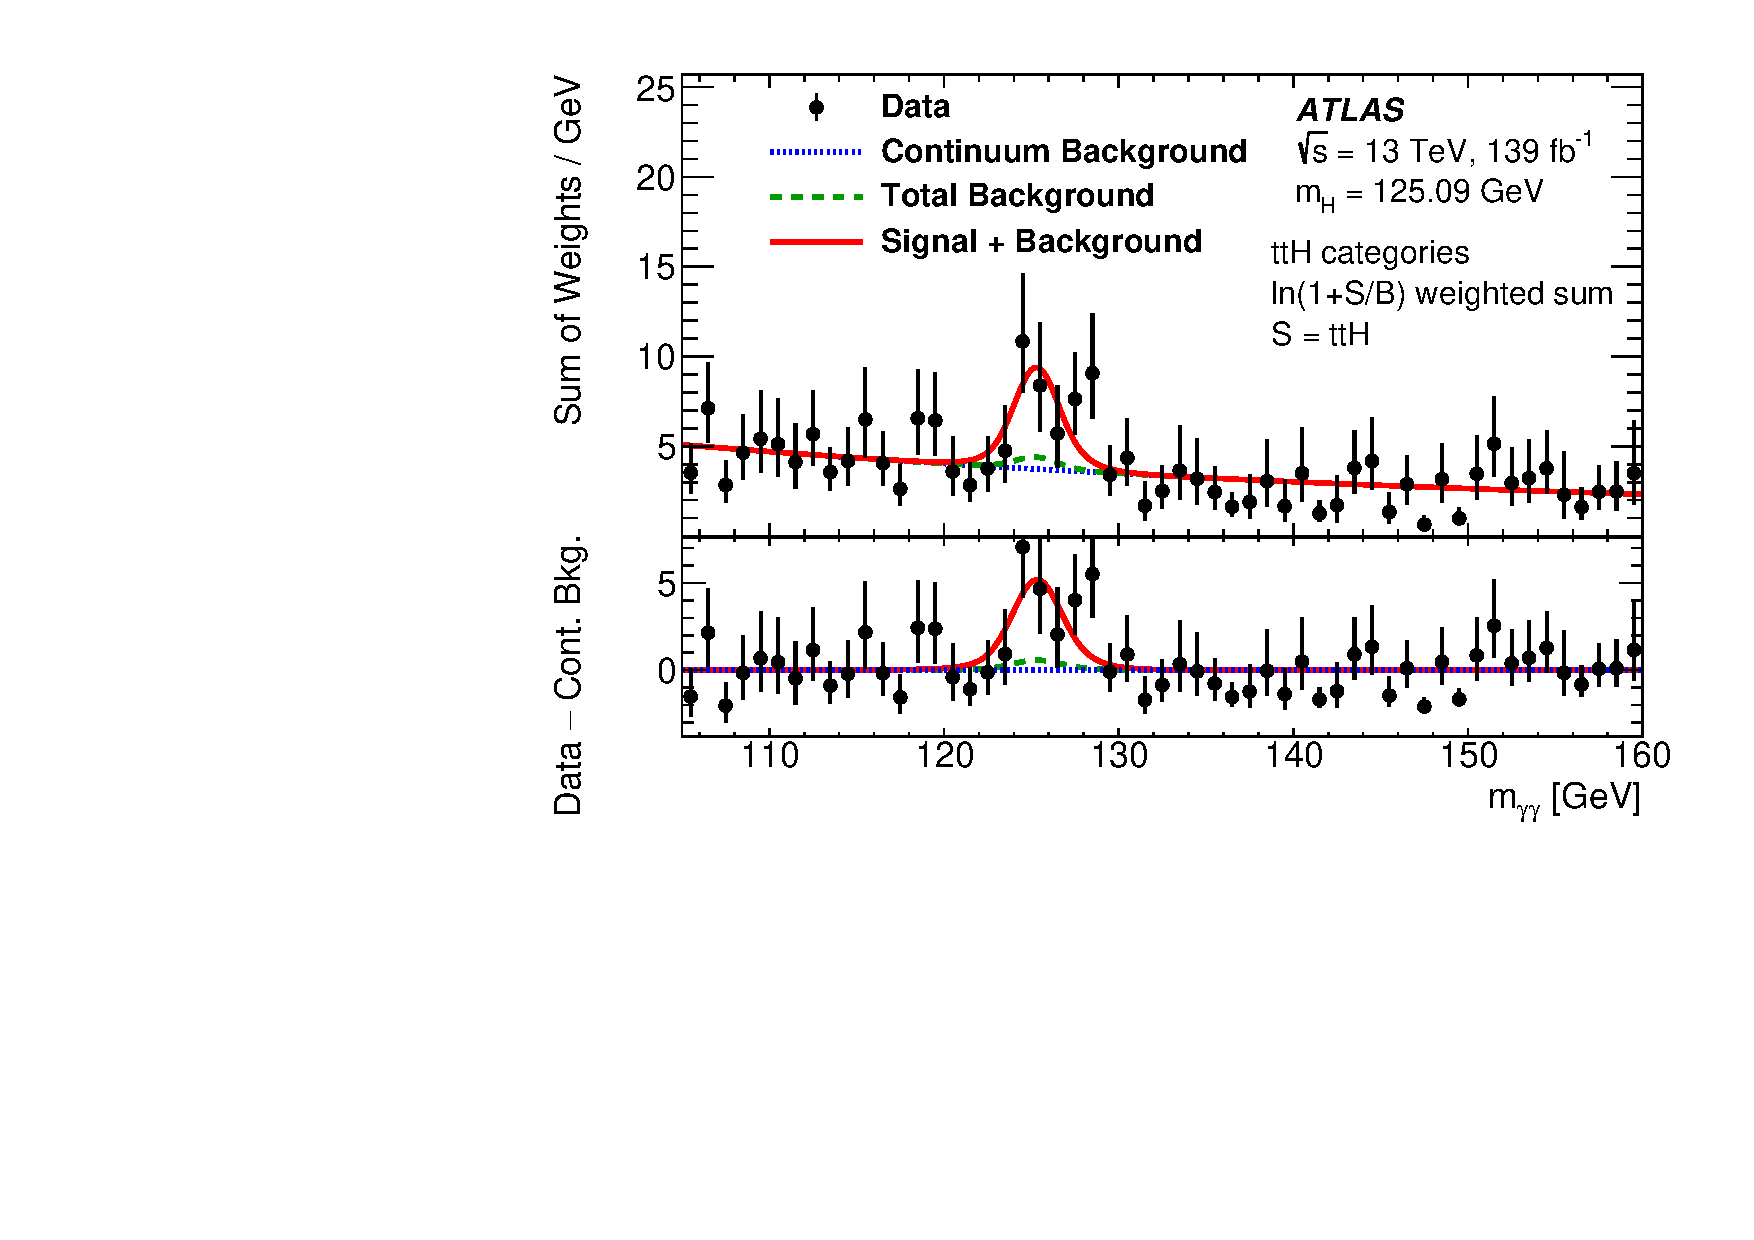
\includegraphics[width=0.6\textwidth]{figures/tth_myy.pdf}
  \caption{\label{fig:myy} Distribution of the diphoton invariant mass in the \ttH\ channel for the latest STXS ATLAS result~\cite{ATLAS_STXS}. The data (dots) are shown together with the sum of the fitted signal plus background (solid line). The blue dotted line represents the sum of the fitted continuum background, while the dashed line combines the contributions of continuum background and other Higgs boson events. The shape of the mass distribution must not be altered by the MVA which is used to discriminate background from signal. The domain adaptation approaches proposed in this text can improve the discrimation power of MVAs while ensuring the MVA does not sculpt the \myy\ spectrum.}
\end{figure}

The most recent ATLAS results that performed many differential cross-section measurements in the \hyy\ channel made use of BDTs to both discriminate between the differential cross-section bins and to separate background from signal processes. One of the main backgrounds in many channels is the continuum diphoton background which is estimated using a functional fit to the \myy\ spectrum (see Figure~\ref{fig:myy} for an example). Due to this background estimation methodology, only variables that were found to have less than a 5\% linear correlation with the \myy\ spectrum were used in the BDT training. The domain adaptation techniques used to improve the photon energy calibration can also be used to ensure that an ML classifier is independent of the \myy\ spectrum. This application of domain adaptation approaches is similar to techniques that have been proposed to decorrelate algorithms to identify substructure within a jet from the mass of the jet, allowing the technique to be used for any mass of a hypothesised BSM particle.

The PI's team will contribute to the ``intermediate'' \hyy\ differential cross-section measurement which was initiated in early 2024 and will use a part of the Run~3 data. The team will focus on re-optimizing the BDTs trained to discriminate between the differential cross-section bins and between signal and the dominant background. This effort will familiarize the team with the existing ML strategy that does not incorporate domain adaptation to ensure that the BDTs are not correlated with the \myy\ spectrum.

Domain adaptation will be applied to the final Run~3 analysis that will use the full Run~3 dataset and that is expected to finalize near the end of the Phase-II shutdown. Using the framework that was developed for the photon ID MVA and energy calibration, the two postdocs and the PI will work in parallel to determine which domain adaptation approach, distance correlation vs adversarial vs feature representation transfer, is optimal for ensuring that the diphoton invariant mass spectrum remains uncorrelated with the signal-to-background MVA (either a BDT or NN). The method that both ensures that the background shape remains unchanged and results in the highest signal significance, which will now take advantage of more variables, will be used in the \hyy\ measurement.

In addition to using domain adaptation to ensure the stability of the \myy\ spectrum, the improved photon ID will be ready to be used in the final Run~3 \hyy\ measurement. The PI's team will focus on optimizing sensitivity to the \tthyy\ which is statistically limited and thus will especially benefit from the improved photon efficiency (reducing the statistical uncertainty by as much as 17\%).

\paragraph{The deliverables associated with the differential cross-section measurement are:}
\begin{itemize}
\item A publication describing the intermediate Run~3 \hyy\ measurement
\item A publication describing the final Run~3 \hyy\ measurement with improved photon ID and background rejection enabled by domain adaptation
\end{itemize}

\subsection{Integrating Domain Adaptation into an ML Framework}

Domain adaptation techniques will be explored and applied across various ML models (BDTs, NNs, and GNNs) and their applications, including object classification, property regression, and event classification. These models will be developed within the SALT framework, which is frequently used within ATLAS, to facilitate the incorporation of domain adaptation into a widely-used machine learning framework. SALT has already been employed to construct ML models for identifying boosted decays to two b-quarks, jets initiated by heavy flavor quarks, $\tau$-leptons, and more. Integrating features into SALT that allow ML models to be decorrelated from specific variables—such as data - MC disparities, pile-up, and others - would reduce uncertainties stemming from discrepancies between recorded and simulated data and equip numerous algorithms for the demanding conditions of the HL-LHC.

Given that the photon ID, photon energy regression, and the \hyy\ signal-to-background ML models incorporating domain adaptation will be partially built using SALT (which predominantly supports GNN-based models), the PI's team will have already embedded domain adaptation techniques within specific SALT implementation. This groundwork will ease the inclusion of a comprehensive domain adaptation framework into SALT. This enhancement will encompass the capability to use manipulated MC data for preliminary tests of domain adaptation strategies and the implementation of various domain adaptation methods. Finally, validation plots will be produced to demonstrate any residual correlations using different techniques, such as distance correlation when adversarial models are the used and the performance of a discriminator trained to differentiate between both domains when distance correlation is employed.

The effort to include domain adaptation, which can require significant computing resources to include during the training of an ML model, into SALT will be aided by synergistic activities within the Argonne ATLAS group. These efforts are geared towards equipping SALT to utilize HPCs, which are expected to drastically cut down training times (preliminary studies indicate a reduction from several days to just a few hours). Leveraging the extensive computing capabilities of HPCs will ensure that the implementation of domain adaptation is not constrained by computational limitations.

\subsection{Timetable of Activities}
\label{sec:timetable}
% Always consider the master timeline:
% https://lhc-commissioning.web.cern.ch/schedule/LHC-long-term.htm

The timetable of activities is shown in Figure~\ref{fig:timetable}.
\begin{figure}[!htbp]
  \centering
  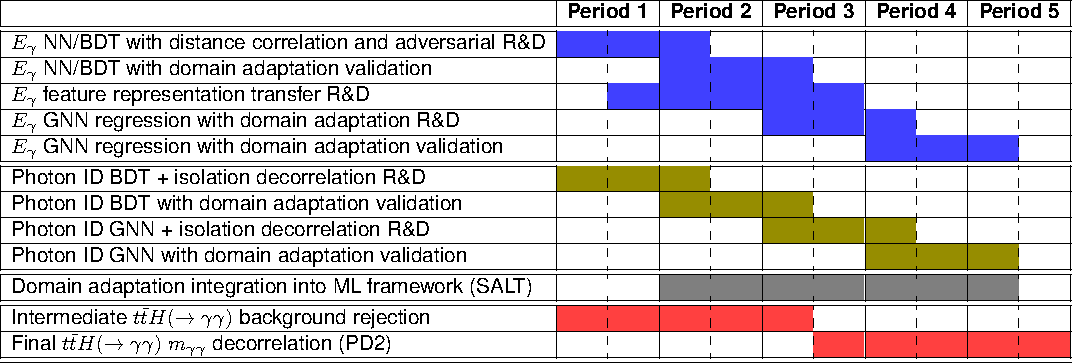
\includegraphics[width=\textwidth]{figures/timeline.pdf}
  \caption{Expected time spent on the work proposed in this text by the PI's team which will consists of two postdocs (at 1.0 FTE each) and about half of the PI's effort. Each period is 12 months long with Period 1 starting on August 1st 2024 and Period 5 ending on July 31st 2029 which is two months after the HL-LHC is slated to start operations (May 2029). The tasks include the application of domain adaptation  techniques to photon energy ($E_{\gamma}$) evaluation. Two established techniques will be studied, distance correlation (DisCo) and adversarial networks (AN), as well as a new technique, feature representation transfer. A subset of domain adaptation techniques which decorrelate the ML model's output from certain features will be used for photon ID and signal-to-background separation in the $\ttbar H$ differential cross-section measurement.
  }
  \label{fig:timetable}
\end{figure}

Below is a summary of the milestones:
\begin{enumerate}
\item Reduction in photon energy resolution uncertainty due to mitigation of data-MC differences using domain adaptation.
\item Multivariate photon ID that is decorrelated from isolation
  \item Updated intermediate \hyy\ differential cross-section measurement using part of the Run~3 dataset
  \item Improved background rejection in \hyy\ enabled by domain adaptation being applied to decorrelate signal-to-background discriminating ML from the \myy\ spectrum
    \item Integration of domain adaptation into ML framework (SALT) for broad use within ATLAS
\end{enumerate}

\subsection{Personnel and Resources}
\label{sec:personnel}
The PI will lead a team to execute the proposed project, involving an average of 2.0 postdoctoral FTEs and contributing 50\% of the PI's effort. These postdocs, fully funded by this award, are slated to begin at the start of the first and second budget periods and will continue through the fifth budget period. Their responsibilities will be divided between implementing domain adaptation strategies and conducting two differential cross-section measurements in the \hyy\ channel.

Additionally, the PI will engage with graduate and undergraduate students on this research through established connections with local universities, supported by several programs. The PI has a track record of mentoring students who participate in programs such as the DOE Office of Science Graduate Student Research program and the Science Undergraduate Laboratory Internships. Furthermore, the Argonne ATLAS Center, which welcomes graduate students from ATLAS collaboration member universities, offers further collaborative opportunities. The PI will work with students from institutions that have existing ties with the Argonne ATLAS group, including NIU, which boasts expertise in photon and Higgs sectors and runs a computing traineeship aligning with the computational demands of this proposal.

For computing needs, the PI will access resources at the Argonne through the Laboratory Computing Resources Center (LCRC), which boasts a significant setup (825 nodes, each with 128 cores) frequently utilized by the Argonne ATLAS group and ATLAS Analysis Center (ATC) university collaborators for preparing ATLAS measurements for publication. Additionally, the PI will use a specialized system at LCRC, comprising six nodes with eight GPUs each, for ML model development. The Argonne ATLAS group holds a renewable computing allocation at LCRC, which can be expanded as required for the proposed tasks. The Argonne Leadership Computing Facility (ALCF) provides further resources and expertise, including both NVIDIA and Intel GPU capabilities, to support the development and training of complex ML models. The PI's team will leverage existing relationships with ALCF experts to develop and refine domain adaptation approaches, crucial to computing scientists, using ALCF resources. Requests for resource allocations will be made as needed to support these activities.

\section{Summary}
Machine learning has become an indispensable tool in HEP, enhancing capabilities in tasks like simulating calorimeter showers, particle identification, and distinguishing between signal and background processes. However, as we approach the era of the HL-LHC with its unprecedented data scale, ML models must become more robust to effectively mitigate the impact of systematic uncertainties on physics measurements.  Domain adaptation approaches like adversarial methods and distance correlation techniques have shown potential in reducing these uncertainties and improving the robustness of models against experimental conditions and data-simulation discrepancies. This proposal outlines a framework to deploy various domain adaptation techniques to enhance physics object ID and property estimation in HEP, aiming to reduce systematic uncertainties and improve model resilience. This effort is crucial for future discoveries in collider physics, especially in the precision era of the High Luminosity-LHC (HL-LHC), where precise measurements are key to probing BSM physics.

\clearpage

\appendix
\part*{Appendices}
% \renewcommand\thesection{\Roman{section}}
\addcontentsline{toc}{part}{Appendices}
\section{Biographical sketch}
\centerline{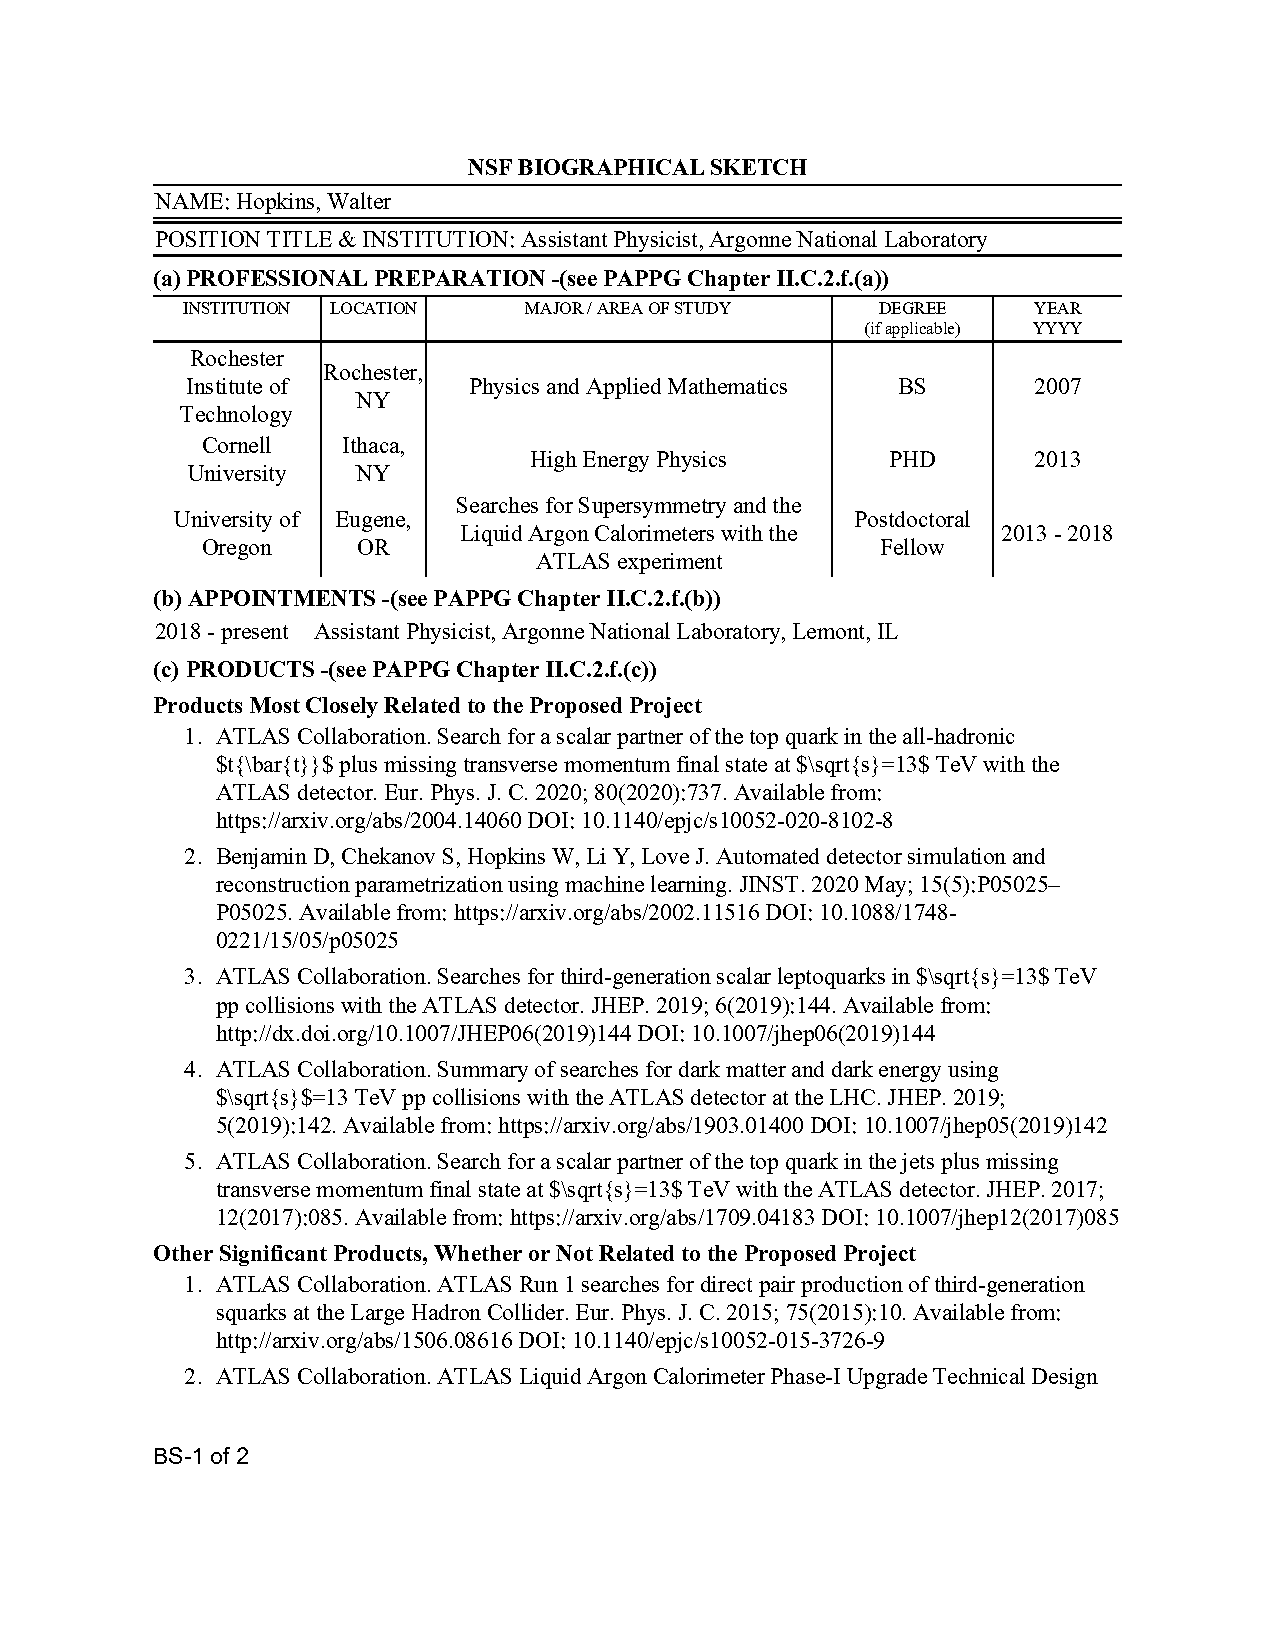
\includegraphics[width=0.99\paperwidth,trim=0 1.73in 0 1.06in,clip]{bioSketch.pdf}}
\includepdf[scale=1,pages=2-,trim=0 1.76in 0 1.06in,clip,pagecommand={}]{bioSketch.pdf}

\clearpage

% \includepdf[scale=.96,pages={1},trim=0 1.5in 0 1.06in,clip,pagecommand=\section{Current and pending support}]{cps_filled.pdf}
% \includepdf[scale=1,pages=2-,trim=0 1.5in 0 1.06in,clip,pagecommand={}]{cps_filled.pdf}
% \clearpage

\printbibliography[title={Bibliography and References},heading=bibnumbered]
\clearpage

\section{Facilities and  other resources}
Argonne offers various resources, including office space for postdocs and potential students as well as several computing resources. The computing resources expected to be utilized include CPU and GPU resources available through the Laboratory Computing Resource Center at Argonne. These resources are expected to be used to produce input data for ML algorithms as well as training the ML algorithms. The PI also plans to use computing resources at the ALCF resources, such as Polaris (which has NVIDIA GPUs) and Aurora (which contains Intel GPUs), via a discretionary allocation. These resources will be used for large-scale training and optimization of the proposed approach.

An additional important resource is the ATLAS experiment at the LHC at CERN. The PI's team will make use of ATLAS data and simulation for the proposed studies and will occasionally travel to CERN to work with international collaborators.

\clearpage

\section{Equipment}
The requested funding will be used to purchase three laptops for the postdocs that the PI will supervise. The combined cost of the three laptops is expected to be \$8,524.

\clearpage

\section{Data management plan}
The majority of the data and code produced will come from the ATLAS experiment. ATLAS has its own data management plan which the PI's team will adhere to; the details of that plan can be found at \url{https://po.usatlas.bnl.gov/programoffice/datamanagementpolicy.php}.

Scientific results that used ATLAS data will be published in a scientific journal or an ATLAS publication note, which will be publicly available on \url{https://arxiv.org/} and \url{https://twiki.cern.ch/twiki/bin/view/AtlasPublic/SimulationPublicResults}, respectively. Figures and tables will be made available in the same way as other ATLAS results, via HEPData (\url{https://www.hepdata.net/}) and ATLAS public pages. 

Additional data that are produced outside of ATLAS for initial ML algorithm development will be stored on the Argonne High Energy Physics divisional nodes in the HDF5 format and will consist of energy deposits in a simplified detector. The generated data are expected to occupy a small fraction of the available data storage on these nodes. Code and configurations used for the development of the algorithm and production of data will be kept at the Argonne Computing, Environment and Life Sciences (CELS) gitlab repository: \url{https://xgitlab.cels.anl.gov/}. Results from these studies, if published, will be publicly available on \url{https://arxiv.org/}. 

\clearpage

\section{Promoting Inclusive and Equitable Research (PIER) Plan}

\clearpage

\section{Recruitment and Retention of Students and Early-stage Investigators}

\clearpage

\section{Other attachments}
There are no other attachments.

\end{document}
